\chapter{Conclusion and Discussion}
\setlength{\parindent}{2.5em}
This project presents a helmet and head detection system trained on a custom dataset using the YOLOv8 architecture, combined with a counting mechanism applied to university CCTV footage. The final model achieved significant accuracy improvements in helmet detection, reaching up to 95\% in our latest version. The double-line counting method effectively reduced duplicate counts and stabilized results, especially for slow-moving or occluded objects. For person and motorbike tracking, the system performed well in low-overlap conditions, providing strong results that demonstrate the system’s potential for practical monitoring and analysis of helmet usage compliance. As for the counting for motorbike and person class, we can implement Bot\_sort tracker as their Yolo model are much for refine allowing us to count regularly through trackers.

\section{Obstacles}

\begin{center}
	\begin{minipage}{0.45\textwidth}
		\centering
		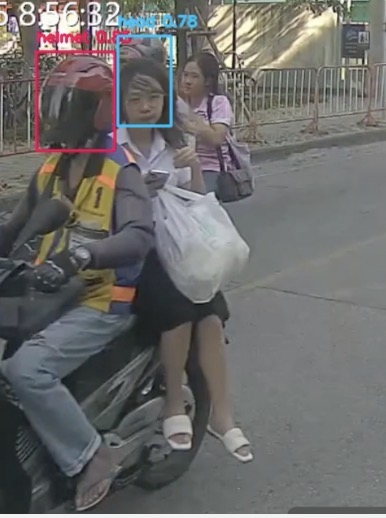
\includegraphics[width=\linewidth]{limitation2.png}
		\vspace{0.5em} % Adjust as needed
		
		\textbf{Figure 5.1}
	\end{minipage}
	\hfill
	\begin{minipage}{0.45\textwidth}
		\centering
		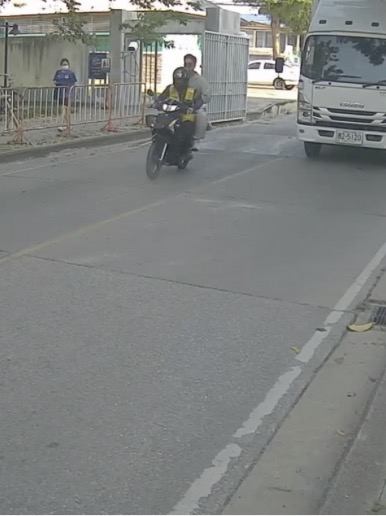
\includegraphics[width=\linewidth]{limitation3.png}
		\vspace{0.5em} % Match the first one
		
		\textbf{Figure 5.2}
	\end{minipage}
\end{center}
\setlength{\parindent}{2.5em}
During system development and testing, the main challenge involved dealing with overlapping bounding boxes, particularly when multiple motorcycles and riders appeared close together, which can be seen in Figure 5.1. This sometimes led to incorrect object counts or detection errors, such as merging two people into one or misidentifying a detection. 

In Figure 5.2 another flaw showing the struggle of tracking system when an object appear to be on another lane, causing it hard for our model to detect an object, especially when it appear to far from the annotation point.


\section{Future Work}
\setlength{\parindent}{2.5em}
In future iterations, the focus will be on improving both the detection model and the tracking accuracy. Training with more diverse and balanced data will help the model generalize better across various environments and video conditions. Further enhancement of the counting and tracking logic is also planned to address issues with ID switching and occlusion. Additionally, while deployment to the university server is not yet complete, it remains a key objective for real-time monitoring in a practical setting. These improvements will support the goal of developing a more accurate, stable, and scalable helmet compliance monitoring system.



